%!TEX root = thesis.tex
\chapter{Analysis of the Monitorability of the TADL2 Timing Constraints}
\label{chapter-TADL2}
%TODO: color diskretisieren

\section{DelayConstraint}
	\label{monitorability_DelayConstraint}
	The \emph{DelayConstraint} is defined as\\[10pt]
	\begin{math}
		\forall x\in source:\exists y\in target: lower\leq y-x\leq upper.
	\end{math}\\[10pt]
	and describes that in the time interval between $lower$ and $upper$ after any $source$ event, there is an $target$ event. Therefore, the state that need to be stored to monitor the \emph{DelayConstraint} is the set of $source$ events, that did not have a matching $target$ event. Updates to this state and outputs of the monitor are done at $source$ and $target$ events and at delay timestamps $upper$ after $source$ events, if there hasn't been a matching $target$ event.\\
	The maximal required storage size of the state depends on the number of $source$ events, which can possibly occur in any time interval of the length $upper$. An example of this worst case situation can be seen in figure~\ref{fig:DelayConstraintWorstCase}. The attributes in this example are $lower=upper=5$, $source=\{1, 1.1, ..., 5.9\}$ and $target=\{6, 6.1, ..., 11\}$. At timestamp 6, all 49 $source$ events must be stored, as they are all required to generate the correct output in this and the following timestamps. At this timestamp, the oldest $source$ event can be removed from the storage, as the matching $target$ event occurs in this timestamp. With every following $target$, the oldest event can be removed from the storage, until every $source$ had its matching $target$ event at timestamp 11.\\
	Because the time domain is understood as real numbers in TADL2, a possibly infinite number of events can be placed in any interval of the length $upper$, therefore the required storage space can grow infinitely. Because the $source$ events are removed from the state, when a matching $target$ event occurs, the required storage space does not grow continuously and infinite resources are only required in worst case scenarios. Therefore, the \emph{DelayConstraint} is \emph{worst case Non-Finite monitorable}.
	\begin{figure}
		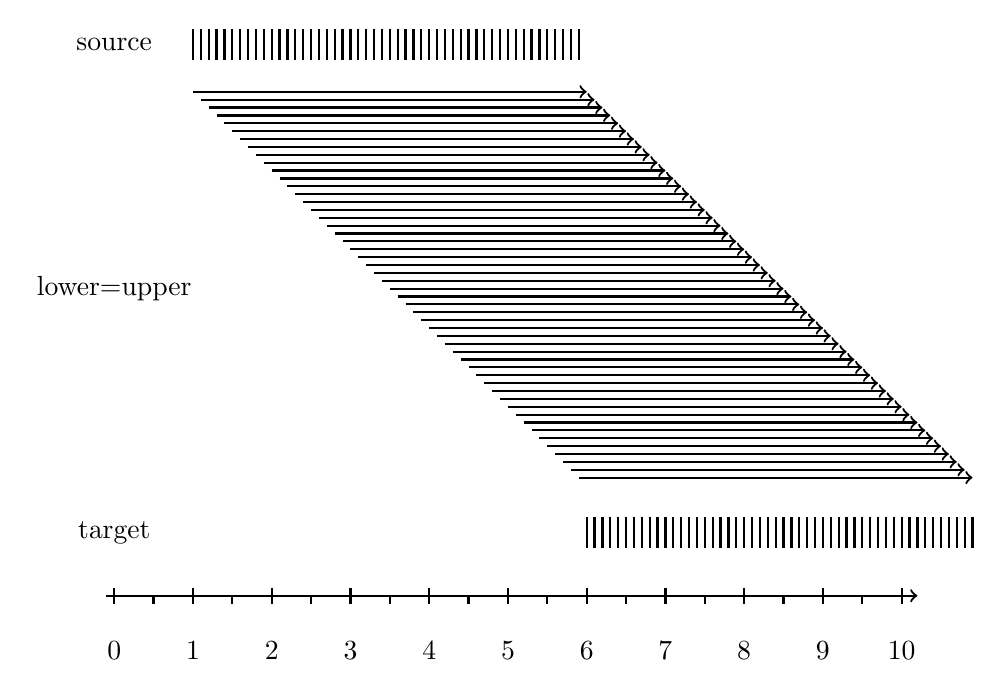
\begin{tikzpicture}[thick]
			\node at (0, 0){source};
			\node at (0, -3.1) {lower=upper};
			\node at (0, -6.2) {target};
			
			%lower = 5, upper = 5
			\foreach \x in {1.0, 1.1, ...,  6}{
				% source
				\draw (\x, 0.2) -- (\x, -0.2);
				% target
				\draw (\x+5, -6) -- (\x+5, -6.4);
			}
			
			% lower/upper
			\foreach \x in {0, 0.1, ..., 5}{
				\draw[->] (1 + \x, -0.6-\x) -- (6+\x, -0.6-\x);
			}
			
			\foreach \y in {-7}{
				\foreach \x in {0, 1, ..., 10}{
					\draw (\x, \y+0.1) -- (\x,  \y-0.1);
					\node at(\x,  \y-0.7) {\x};
				}
				\foreach \x in {0.5, 1.5, ..., 9.5}
				\draw (\x, \y) -- (\x, \y-0.1);
				\draw[->] (-0.1, \y) -- (10.2, \y);
			}
		\end{tikzpicture}
		\caption{\emph{DelayConstraint} or \emph{StrongDelayConstraint}  with $lower=upper=5$}
		\label{fig:DelayConstraintWorstCase}
	\end{figure}
	

	
\section{StrongDelayConstraint}
	The difference between the \emph{DelayConstraint} and the \emph{StrongDelayConstraint} is, that for every $source$ event, there must be exactly one matching $target$ event in the \emph{StrongDelayConstraint}. Therefore, the state of the monitor is nearly the same, as every $source$ event, that did not have a matching $target$ event yet, must be stored. Therefore, the only difference is, when these $source$ events can removed from state and the \emph{StrongDelayConstraint} is \emph{worst case Non-Finite monitorable}, like the \emph{DelayConstraint}.

\section{RepeatConstraint}
	The \emph{RepeatConstraint} defines the time distance between each event and its $span^{th}$ successor. Therefore, the state, that must be stored, consists of the timestamps of the $span+1$ latest events. The state is updated at every event, the oldest stored event is removed and the timestamp of the current event is placed in the storage. The output function checks, if the time distance between the oldest stored event and the current timestamp is between $lower$ and $upper$. To monitor this constraint, a single delay is required, because a missing event, or an event that occurs too late, would not be determined in the right timestamp.\\
	As the memory requirements are fix ($span+1$ timestamps must be stored) and the state transition and output function can be programmed in a way that they are in  $\mathcal O(1)$, the \emph{RepeatConstraint} is finite monitorable with delay.

\section{RepetitionConstraint}
	The \emph{RepetitionConstraint} is defined as\\[10pt]
		$RepetitionConstraint(s, lower, upper, span, jitter)$\\
		$\equiv \exists X\subset \mathbb{T}: RepeatConstraint (X, lower, upper, span)$\\
		\hspace{7cm}$\land$ $StrongDelayConstraint(X, s, 0, jitter)$\\[10pt]
	The elements of set $X$ follow the RepeatConstraint and the events, which should be monitored, are following in an interval of the length $jitter$ after the elements of $X$. For each element of $X$, there is exactly one event and vice versa.\\
	The monitoring algorithm for this constraint, which will be explained in detail in \ref{chapter-implementation}, stores the upper and lower bounds for the next $span$ elements of $X$.
	These borders are stored in a list and calculated by\\[10pt]
	$lowerBound:= List\_append(last(List\_tail(LowerBound), s), lowerBoundNow + lower)$ for the lower bound and\\
	$upperBound:= List\_append(last(List\_tail(UpperBound), s), upperBoundNow + upper)$.\\[10pt]
	The oldest item in these lists (the head of these lists) are removed and the newly calculated bounds for the $span$ next element of $X$ is inserted. $lowerBoundNow$ and $upperBoundNow$ are the describing the limitations of the element of $X$ right before the current event. They are calculated using the list mentioned above and the timestamp of the current event by the following definition:\\[10pt]
	$lowerBoundNow:= max(List\_head(last(LowerBoundX, s)), time(s)-jitter)$\\
	$upperBoundNow:= min(List\_head(last(UpperBoundX, s)), time(s))$\\[10pt]
	If the timestamp of the current event is between $lowerBoundNow$ and $upperBoundNow$, the output of the monitor is $true$, in any other case, or when the delay ran out, it is $false$.\\
	The size of these lists has a fixed upper limit ($span$) and the state transition and output functions are in $\mathcal{O}(1)$, therefore the \emph{RepetitionConstraint} is finite monitorable with delay.
	
\section{SynchronizationConstraint}
	The \emph{SynchronizationConstraint} describe groups of event sets, which events occur in common clusters. Each of these sets must have at least one event in each of these intervals. Any events, that lay outside of these intervals are prohibited.\\
	Figure~\ref{fig:SynchronizationConstraintWorstCase}, which is similar to the example for the \emph{DelayConstraint}, shows an example of this constraint, which is an worst case scenario in terms of monitoring. The $tolerance$ interval is 5 timestamps long, the event set $s_1$ contains the events $\{1, 1.1, ..., 5.9\}$ and $s_2$ is containing $\{6, 6.1, ..., 11\}$. Each of the events of $s_1$ must be stored until the end of the $tolerance$ interval, otherwise it would be impossible to check the constraint correctly. Like described in chapter~\ref{monitorability_DelayConstraint}, an infinite number of events can be placed in this interval, therefore infinite memory resources are needed. Because the required storage space is not growing continuously, as the stored events can be removed at the end of the $tolerance$ interval, the \emph{SynchronizationConstraint} is worst case Non-Finite monitorable.\\
	\\
	It should be noted, that the illustration of the constraint in figure~\ref{fig:SynchronizationConstraintWorstCase} may be misleading, because the $tolerance$ intervals are only shown after the events of $s_1$, not after the events of $s_2$. Every implementation of a monitor for this constraint must also store the events of $s_2$ for the length of $tolerance$, as they could be important for events following after them.
	\begin{figure}
		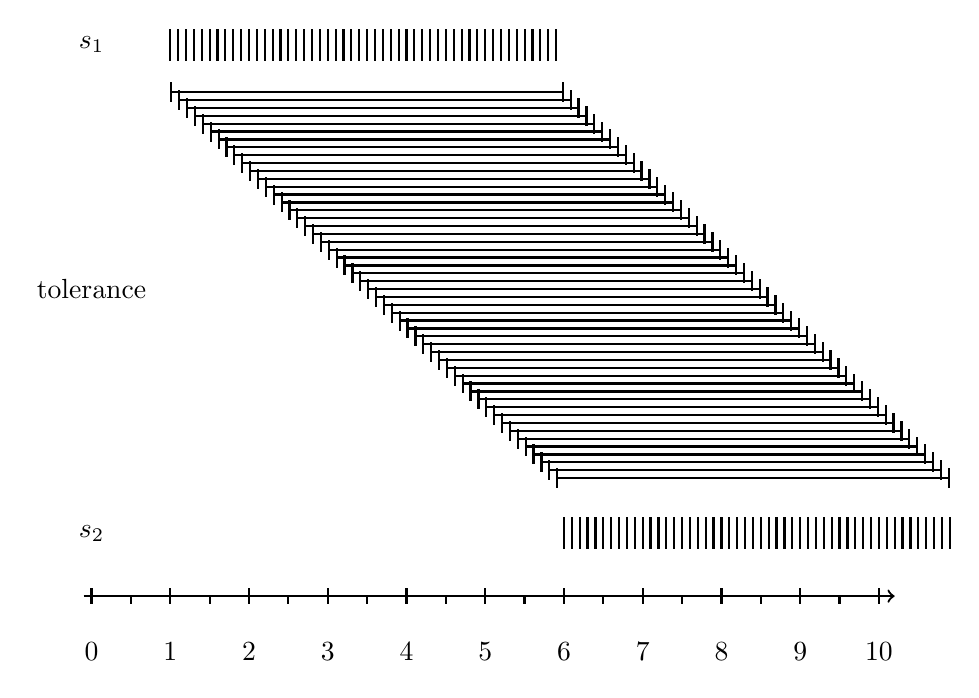
\begin{tikzpicture}[thick]
		\node at (0, 0){$s_1$};
		\node at (0, -3.1) {tolerance};
		\node at (0, -6.2) {$s_2$};
		
		\foreach \x in {1.0, 1.1, ...,  6}{
			% s_1
			\draw (\x, 0.2) -- (\x, -0.2);
			% s_2
			\draw (\x+5, -6) -- (\x+5, -6.4);
		}
		
		% tolerance
		\foreach \x in {0, 0.1, ..., 5}{
			\draw[|-|] (1 + \x, -0.6-\x) -- (6+\x, -0.6-\x);
		}
		
		\foreach \y in {-7}{
			\foreach \x in {0, 1, ..., 10}{
				\draw (\x, \y+0.1) -- (\x,  \y-0.1);
				\node at(\x,  \y-0.7) {\x};
			}
			\foreach \x in {0.5, 1.5, ..., 9.5}
			\draw (\x, \y) -- (\x, \y-0.1);
			\draw[->] (-0.1, \y) -- (10.2, \y);
		}
		\end{tikzpicture}
		\caption{\emph{SynchronizationConstraint} or \emph{StrongSynchronizationConstraint}  with $tolerance=5$}
		\label{fig:SynchronizationConstraintWorstCase}
	\end{figure}
	
	
\section{StrongSynchronizationConstraint}
	The difference between the \emph{StrongSynchronizationConstraint} and the \emph{SynchronizationConstraint} is, that in the StrongSynchronizationConstraint, only one event per event set is allowed in each synchronization cluster. Therefore, this constraint can be classified as worst case Non-Finite monitorable with the same argumentation as the previous constraint.
	
	
\section{ExecutionTimeConstraint}
	The \emph{ExecutionTimeConstraint} ensures that the time distance between $stop$ and $start$ events, not counting interruptions (which are specified by $preempt$ and $resume$ events).\\
	Under the assumption that the input events are in logical order (every execution is started by an $start$ event and finished by an $stop$ event, every $preempt$ event is directly followed by an $resume$ event and no $preempt$ or $resume$ events occur outside of the intervals spanned by $start$ and $stop$ events), three time values must be stored, to monitor this constraint. First, the timestamp of the latest $start$ event. Second, the sum of the timestamps of the $preempt$ events, reseted by every $start$ event and third, the sum of the timestamps of the $resume$ events, also reseted by every $start$ event.\\
	For the output function, the run time can be calculated by\\ $runtime = time(now) - start - (sum(resume)-sum(preempt))$.\\ At any event, this value must smaller or equal to $upper$ and at $stop$ events, additionally the runtime must be greater or equal to $upper$. \\
	%TODO Delay
	Therefore the required storage space is fixed, also the runtime of the state transition and output function is in $\mathcal{O}(1)$, therefore the \emph{ExecutionTimeConstraint} is finite monitorable with delay.


\section{OrderConstraint}
	The \emph{OrderConstraint} describes, that an $i^{th}$ $target$ event must exist, if an $i^{th}$ $source$ event exists and that the $i^{th}$ $target$ event occurs after the $i^{th}$ $source$ event. Because it is possible that an arbitrary large number of $source$ events occur before the first $target$ occurs, a possibly infinite large number must be stored, which requires infinite memory resources. As this is only a worst case scenario and the size of the stored number can be decreased, when a $target$ event occurs, the \emph{OrderConstraint} is worst case non-finite monitorable.
	
\section{ComparisonConstraint}
	The \emph{ComparisonConstraint} defines an ordering relation between two single timestamps. Therefore, no additional storage is needed and as the relations ($\leq, <, \geq, >, =$) can be decided in constant time for discrete timestamps, this Constraint is finite monitorable.
	
\section{SporadicConstraint}
	The \emph{SporadicConstraint} is defined via the \emph{Repetition-} and \emph{RepeatConstraint} without introducing any new timestamps in the definition of the \emph{SporadicConstraint}. These Constraints are finite monitorable with delay, therefore the \emph{SporadicConstraint} is also finite monitorable with delay.
	
\section{PeriodicConstraint}
	The \emph{PeriodicConstraint} is special application of the \emph{SporadicConstraint}, therefore it is also finite monitorable with delay.
	
\section{PatternConstraint}
%	The \emph{PatternConstraint} is defined as\\[10pt]
%	\begin{math}
%		\exists X: PeriodicConstraint(X, period, 0, 0)\\
%		\text{\hspace{.5cm}} \land \forall i: DelayContraint(X, event, offset_i, offset_i+jitter)\\
%		\text{\hspace{.5cm}} \land RepeatConstraint(event, minimum, \infty, 1)
%	\end{math}\\[10pt]
%	The events ($event$), which are given as attribute, follow after the elements of $X$, a set of timestamps, which are repeated strictly periodic. The distance between the elements of 
%	%TODO (DelayConstraint<->StrongDelayConstraint)
%
%	
%	This constraint can be monitored by storing upper and lower limits of the 
	
	
\section{ArbitraryConstraint}
	The \emph{ArbitraryConstraint} is defined as combination of the \emph{RepeatConstraint}:\\[10pt]
	\begin{math}
		ArbitraryConstraint(event, minimum_1, ..., minimum_n, maximum_1, ..., maximum_n)\\
		\Leftrightarrow \forall i\in{1, ..., n}: RepeatConstraint(event, minimum_i, maximum_i, i).
	\end{math}\\[10pt]
	The \emph{RepeatConstraint} is finite monitorable with delay, therefore the \emph{ArbitraryConstraint} is also finite monitorable with delay.
	
\section{BurstConstraint}
	The \emph{BurstConstraint} is defined as combination of the \emph{RepeatConstraint}:\\[10pt]
	\begin{math}
		RepeatConstraint(event, length, \infty, maxOccurrences)\\
		\text{\hspace{.5cm}}\land RepeatConstraint(event, minimum, \infty, 1)
	\end{math}\\[10pt]
	The \emph{RepeatConstraint} is finite monitorable with delay, therefore the \emph{BurstConstraint} is also finite monitorable with delay.
	
\section{EventChain}
	\emph{EventChains}, which are required for the following constraints, are defined as sets of $stimulus$ and $response$ events. The events have an color attribute, which describes the causal connection individual events of $stimulus$ and $response$. It is required, that any $stimulus$ event with a specific color must occur before the first $response$ event with the same color. The datatype of this attribute is not specified, except that it may be infinite and an equality test exist.\\
	Monitoring this property is difficult, because it is required to store every color which has occurred in $response$. The reason for this can be seen in figure~\ref{fig:colorExample}. In the interval between the timestamps 1 and 2, there are 5 events of different colors in $stimulus$. Their counterparts in $response$ occur in the interval between 4 and 5. In timestamp 6, there is an event in $response$ with a color, that hasn't been used in $stimulus$ before, therefore this color may not be used in $stimulus$ anymore. To check this for further events in $stimulus$, it is required to know any color that previously occurred in $response$.\\
	The memory consumption to monitor this is growing continuously with any event that introduces a new color in $response$, therefore any constraint, that requires the color attribute (\textbf{\emph{ReactionConstraint, AgeConstraint, OutputSynchronizationConstraint, InputSynchronizationConstraint}}) is always non-finite monitorable.
	\begin{figure}
		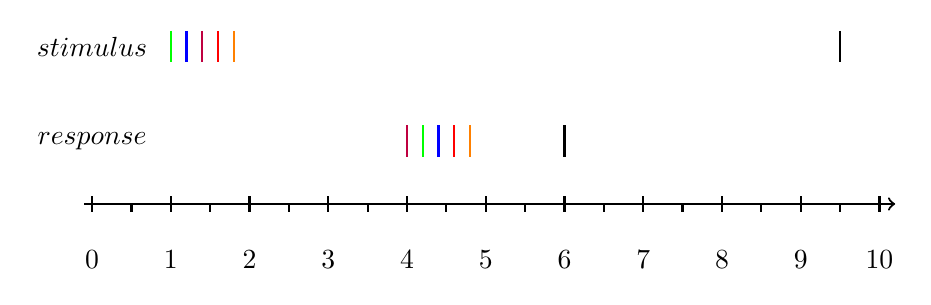
\begin{tikzpicture}[thick]
		\node at (0, 0){$stimulus$};
		\node at (0, -1.2) {$response$};
		%stimulus
		\foreach \x in {0}{
			\draw[green]	(\x + 1  , 0.2) -- (\x + 1  , -0.2);
			\draw[blue]		(\x + 1.2, 0.2) -- (\x + 1.2, -0.2);
			\draw[purple]	(\x + 1.4, 0.2) -- (\x + 1.4, -0.2);
			\draw[red]		(\x + 1.6, 0.2) -- (\x + 1.6, -0.2);
			\draw[orange]	(\x + 1.8, 0.2) -- (\x + 1.8, -0.2);
		}
		%\draw[green]	(8  , 0.2) -- (8 , -0.2);
		\draw[black]	(9.5  , 0.2) -- (9.5 , -0.2);
		%response
		\foreach \x in {3}{
			\draw[purple]	(\x + 1  , -1) -- (\x + 1  , -1.4);
			\draw[green]		(\x + 1.2, -1) -- (\x + 1.2, -1.4);
			\draw[blue]	(\x + 1.4, -1) -- (\x + 1.4, -1.4);
			\draw[red]		(\x + 1.6, -1) -- (\x + 1.6, -1.4);
			\draw[orange]	(\x + 1.8, -1) -- (\x + 1.8, -1.4);
		}
		\draw[black]	(6, -1) -- (6, -1.4);
		\foreach \y in {-2}{
			\foreach \x in {0, 1, ..., 10}{
				\draw (\x, \y+0.1) -- (\x,  \y-0.1);
				\node at(\x,  \y-0.7) {\x};
			}
			\foreach \x in {0.5, 1.5, ..., 9.5}
			\draw (\x, \y) -- (\x, \y-0.1);
			\draw[->] (-0.1, \y) -- (10.2, \y);
		}
		\end{tikzpicture}
		\centering
		\caption{Color attribute }
		\label{fig:colorExample}
	\end{figure}
	
%\section{ReactionConstraint}
%	The \emph{ReactionConstraint} is defined as:
%	\\[10pt]
%	\begin{math}
%		\forall x\in scope.stimulus: \exists y\in scope.response:\\
%		\text{\hspace{.5cm}}x.color=y.color\\
%		\text{\hspace{.5cm}}\land (\forall y'\in scope.response: y'.color=y.color\Rightarrow y\leq y')\\
%		\text{\hspace{.5cm}}\land minimum \leq y-x \leq maximum
%	\end{math}\\[10pt]
%	%For every event $x$ in $scope.stimulus$, there is an event $y$ in $scope.response$ with the same color. The distance between $x$ and $y$ is specified by $minimum$ and $maximum$.
%	The third line is the most relevant for the classification of monitorability. It says, that additional events in $scope.response$ with the same color of $y$ must occur at or after $y$. Other restrictions to additional events in $scope.response$ are not defined.\\
%	\ref{fig:WorstCaseReactionConstraint} visualizes, where this leads to problems in terms of monitoring. Between the timestamps 1 and 7, there are many events with different colors in $scope.response$ and the constraint is satisfied. In timestamp 8, there is an event in $scope.stimulus$ that has a color that matches with one of the $scope.response$ events, therefore the constraint is not fulfilled anymore.\\
%	The Example shows, that every color of the events that have occurred in $scope.response$ must be stored, to monitor the constraint correctly. Any new $scope.response$ event with a new color will extend the required storage space, but it is not possible to release this storage and still monitor the constraint correctly, therefore the memory requirements grows continuously. The definition of the color attribute of events says, that there is an infinite number of possible colors, therefore infinite memory resources are required for this constraint.
%	These characteristics show that this constraint is always non-finite monitorable.
%	\begin{figure}
%		\begin{tikzpicture}[thick]
%			\node at (0, 0){$stimulus$};
%			\node at (0, -1.2) {$response$};
%			%stimulus
%			\draw[green] (8, 0.2) -- (8, -0.2);
%			%response
%			\foreach \x in {0, ..., 5}{
%				\draw[green]	(\x + 1  , -1) -- (\x + 1  , -1.4);
%				\draw[blue]		(\x + 1.2, -1) -- (\x + 1.2, -1.4);
%				\draw[purple]	(\x + 1.4, -1) -- (\x + 1.4, -1.4);
%				\draw[red]		(\x + 1.6, -1) -- (\x + 1.6, -1.4);
%				\draw[orange]	(\x + 1.8, -1) -- (\x + 1.8, -1.4);
%			}
%			\foreach \y in {-2}{
%				\foreach \x in {0, 1, ..., 10}{
%					\draw (\x, \y+0.1) -- (\x,  \y-0.1);
%					\node at(\x,  \y-0.7) {\x};
%				}
%				\foreach \x in {0.5, 1.5, ..., 9.5}
%				\draw (\x, \y) -- (\x, \y-0.1);
%				\draw[->] (-0.1, \y) -- (10.2, \y);
%			}
%		\end{tikzpicture}
%		\caption{ReactionConstraint - Example with additional events and $minimum=maximum=3$}
%		\label{fig:WorstCaseReactionConstraint}
%	\end{figure}
%%TODO response events before stimulus allowed?
%	
%\newpage
%\section{AgeConstraint}
%	The \emph{AgeConstraint} is defined as \\[10pt]
%	\begin{math}
%	\forall y\in scope.response: \exists x\in scope.stimulus:\\
%	\text{\hspace{.5cm}}x.color=y.color\\
%	\text{\hspace{.5cm}}\land (\forall x'\in scope.stimulus: x'.color=x.color\Rightarrow x'\leq x)\\
%	\text{\hspace{.5cm}}\land minimum \leq y-x \leq maximum
%	\end{math}\\[10pt]
%	It is a turned around counterpart to the \emph{ReactionConstraint}, where each event $y$ of $scope.response$ is preceded by an event $x$ in $scope.stimulus$ with matching color. The distance between these events is defined by the attributes $minimum$ and $maximum$. After the latest event $x$, that matches color with $y$ and is in the right distance (hence after $y-minimum$), no more events with this color are allowed. To monitor this property correctly, it is necessary to store, amongst other things, every color of events, that occurred in $scope.response$.  Figure~\ref{fig:WorstCaseAgeConstraint} visualizes this. In the interval from 5 to 6 there are 5 events in $scope.response$, their matching $scope.stimulus$ events are in the interval from 2 to 3. In timestamp 10, there is an event in $scope.stimulus$, which has a color that matches with an color, that has already been used in $scope.response$. The \emph{AgeConstraint} is not satisfied anymore after this, but to find that out, it is required to know every color, which  has already been used in $scope.response$. Like in the \emph{ReactionConstraint}, the memory requirements for this is growing continuously, therefore the \emph{AgeConstraint} is always non-finite monitorable.
%	
%	\begin{figure}
%		\begin{tikzpicture}[thick]
%		\node at (0, 0){$stimulus$};
%		\node at (0, -1.2) {$response$};
%		%stimulus
%		\draw[green]	(2  , 0.2) -- (2  , -0.2);
%		\draw[blue]		(2.2, 0.2) -- (2.2, -0.2);
%		\draw[purple]	(2.4, 0.2) -- (2.4, -0.2);
%		\draw[red]		(2.6, 0.2) -- (2.6, -0.2);
%		\draw[orange]	(2.8, 0.2) -- (2.8, -0.2);
%		
%		\draw[green]	(10, 0.2) -- (10, -0.2);
%		
%		\foreach \x in {0, 0.1, 0.2, 0.3, 0.4}
%			\draw[<-] (2+\x+\x, -0.5-\x) -- (5+\x+\x, -0.5-\x);
%		%response
%		\draw[green]	(5  , -1) -- (5  , -1.4);
%		\draw[blue]		(5.2, -1) -- (5.2, -1.4);
%		\draw[purple]	(5.4, -1) -- (5.4, -1.4);
%		\draw[red]		(5.6, -1) -- (5.6, -1.4);
%		\draw[orange]	(5.8, -1) -- (5.8, -1.4);
%		\foreach \y in {-2}{
%			\foreach \x in {0, 1, ..., 10}{
%				\draw (\x, \y+0.1) -- (\x,  \y-0.1);
%				\node at(\x,  \y-0.7) {\x};
%			}
%			\foreach \x in {0.5, 1.5, ..., 9.5}
%			\draw (\x, \y) -- (\x, \y-0.1);
%			\draw[->] (-0.1, \y) -- (10.2, \y);
%		}
%		\end{tikzpicture}
%		\caption{AgeConstraint - Example with additional events and $minimum=maximum=3$}
%		\label{fig:WorstCaseAgeConstraint}
%	\end{figure}
%	
%
%\section{OutputSynchronizationConstraint}
%	The \emph{OutputSynchronizationConstraint} is defined as\\[10pt]
%	\begin{math}
%		\forall x\in scope_1.stimulus: \exists t: \forall i: \exists y\in scope_i.response:\\
%			\text{\hspace{.5cm}} x.color = y.color\\
%			\text{\hspace{.5cm}}\land (\forall y'\in scope_i.response: y'.color=y.color \Rightarrow y\leq y')\\
%			\text{\hspace{.5cm}}\land 0\leq y-t\leq tolerance,
%	\end{math}\\[10pt]
%	where every $scope_i$ has the same $stimulus$ events.\\
%	Each $scope_1.stimulus$ event $x$ has an event $y$ in every $scope_i.response$ with the same color. This event $y$ is the first occurrence of this color in $scope_i.response$ and the $y$-events of all $scope_i.response$ do not lay more than $tolerance$ time apart.\\
%	A worst case scenario can be constructed, in which any number of events with different colors is placed in $scope_1.stimulus$. To monitor this constraint correctly, the color of all of these events must be stored, until the $response$ event with matching colors occur. Because an infinite number of colors is possible, infinite storage space is needed to monitor this constraint correctly. The colors of the events can be removed from the storage, after the first occurrence of them in the $response$ events, therefore the required memory is not growing continuously and the constraint is worst case Non-Finite monitorable.
%	
%\section{InputSynchronizationConstraint}
%	The \emph{InputSynchronizationConstraint} is defined as\\[10pt]
%	\begin{math}
%		\forall y\in scope_1.response: \exists t: \forall i: \exists x\in scope_i.stimulus:\\
%		\text{\hspace{.5cm}} x.color = y.color\\
%		\text{\hspace{.5cm}}\land (\forall x'\in scope_i.stimulus: x'.color=x.color \Rightarrow x\leq x')\\
%		\text{\hspace{.5cm}}\land 0\leq x-t\leq tolerance
%	\end{math}\\[10pt]
%	and offers an turned around counterpart to the \emph{OutputSynchronizationConstraint}. The synchronized event clusters occur in the $scope_i.stimulus$ events and the latest events of them must be part of the synchronization. Like for the \emph{OutputSynchronizationConstraint} a worst case scenario, where an possibly infinite number of event colors must be stored, can be constructed, by putting a possibly infinite large number of synchronized events into the $scope_i.stimulus$ event sets, before the first event occurs in $scope_1.response$. Similar to the  \emph{OutputSynchronizationConstraint}, the colors of these events must be stored, until they are released by the $response$ events with a matching color, therefore infinite memory resources are required to monitor this constraint correctly and the \emph{InputSynchronizationConstraint} is worst case Non-Finite monitorable.